\subsection{Akkumulator}
\label{sec:Valid_Batterie}

\subsubsection{ADC Messung der Batteriespannung}

Die Spannungsmessung inkl. Korrekturfaktor für den Spannungsteiler wird mit Hilfe einer Source Measuring Unit überprüft. Die Dabei entstandenen Werte sind in der Abbildung \ref{pic:ADC_Spannung_Graph} geplottet.

\begin{figure}[H]
	\centering
	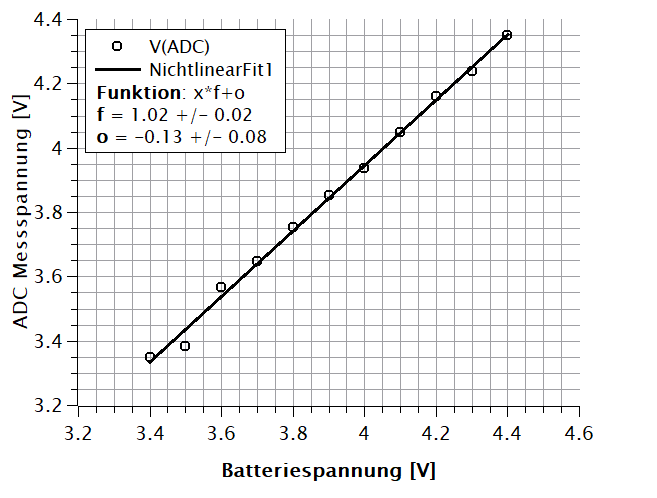
\includegraphics[width=0.8\linewidth]{ADC_Spannung_Graph}
	\caption{Akkumulatorspannung im Vergleich mit der gemessenen Spannung am ADC}
	\label{pic:ADC_Spannung_Graph}
\end{figure}

Auf die gemessenen Werte liefert ein linearer Fit folgende Erkenntnis.
Die Messwerte sind durchschnittlich um $V_{offset}=-130\si{mV}$ zu gering.
Zu einem Teil sind die Abweichungen auf die Widerstandtoleranzen des Spannungsteilers zurückzuführen.
Ein weiterer Einflussfaktor hat die Batteriespannung selber, da diese durch den BQ2409x nicht konstant gehalten wird. Auch das Fehlen einer Filterschaltung für das ADC Signal verschlechtert die Messergebnisse.

Verwendetes Messgerät:

Agilent N6705B (Prüfmittel Nr. \texttt{MSZ-M-0064}) auf Channel 1 mit Strombegrenzung $I_{max}=600\si{mA}$.

Verwendeter Prüfling:

\textit{DSP-Board Nr. 5}

\todo{SB - Verweis auf einen Zielwert. zb. Eingehalten auf +- 100mV genau blabla reicht um Low Voltage zu detektieren}

\subsubsection{Ladestrombegrenzung}

\todo{Diesen Abschnitt nochmals gut durchlesen und auf vollstädnigkeit überprüfen -ich war müde}

Zum Testen der Strombegrenzung des BQ2409x wurde das DSP Board gemäss dem Messschema in Abbildung \ref{pic:SMU_Messung} an angeschlossen.
Dabei erzeugt die SMU mit den Parametern aus Tabelle \ref{tab:SMU_Params_Current} zusätzlich eine Spannung vom $U_{SMU}=+0.1\si{V}$.
Zum Ändern der Ladestromlimite wird der GPIO \texttt{PB14} (Set $I_{LIM}$) getogglet.
\textit{R16} hat einen Wert von $R_{16}=2.7k\Omega$, was einen Ladestrom von $I_{charge}=200\si{mA}$ einstellt.

\begin{figure}[H]
	\centering
	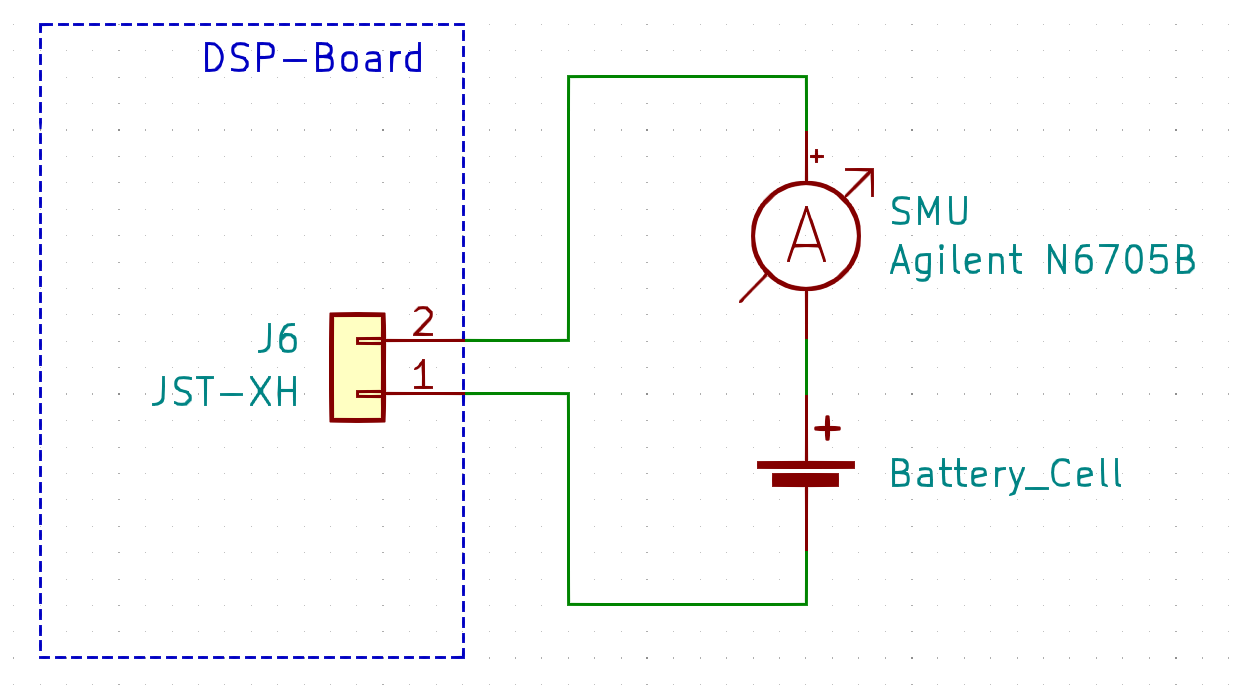
\includegraphics[width=0.5\linewidth]{SMU_Messung}
	\caption{Messschaltung zur Bestimmung des Ladestroms durch Serieschaltung einer SMU}
	\label{pic:SMU_Messung}
\end{figure}

\begin{table}[H]
	\begin{tabular}{|l|l|l|c|c|}
		\hline
		Messgerät      & Kanal & Prüffmittelnummer & Spannungsbereich & Strombegrenzung \\ \hline
		Agilent N6705B & CH1   & MSZ-M-0064        & 0.1V      & 0.5A            \\ \hline
	\end{tabular}
	\caption{Parameter der SMU}
	\label{tab:SMU_Params_Current}
\end{table}

\begin{table}[H]
	\centering
	\begin{tabular}{|c|r|r|r|}
		\hline
		\texttt{SET\_I\_LIM} & $I_{bat}[\si{mA}]$ (erwartet) &  $I_{bat}[\si{mA}]$ (on) & $I_{bat}[\si{mA}]$ (off) \\ \hline
		\texttt{HIGH} & $500$ & $200$ & $145$ \\ \hline
		\textit{floating} (0.9V) & (\textit{set by R16}) $200$ & $200$ & $145$ \\ \hline
		\texttt{LOW} & $100$ & $200$ & $145$ \\ \hline
	\end{tabular}
	\label{tab:Icharge_Results}
	\caption{Gemessene Ladeströme beim Akku}
\end{table}

\todo{LAdestrom Tabelle wird nicht referenziert?? WTF??}

Die Resultate aus der Tabelle \ref{tab:Icharge_Results} zeigen, dass bei eingeschaltetem STM32 ein Betriebsstrom von ca. $55\si{mA}$ entfallen.
Bei ausgeschalteter Schaltung beträgt der Ladestrom, wie erwartet $I_{charge}=200\si{mA}$.
Jedoch ist dieser in jedem Betriebsfall gleich hoch. Der Zustand vom \texttt{ISET2} Pin hat keinerlei Einfluss auf die Strombegrenzung.
Diese Abweichung kann aktuell nicht erklärt werden.




